% ================================================================
%  第 2 章 所有那些矩形 (All those rectangles)
%  依据原书 PDF 第 21--41 页译出；编号审计见文件末尾注释
% ================================================================

\chapter{所有那些矩形}

\epigraph{在数学中, 一如在生活中, 常常更便利的做法是只积分正的部分.}{Antoni Zygmund}

\section{一般事实}

给定测度空间 $(X, \mathrm{d}\mu)$ 与一族由有限测度可测子集对组成的族 $\mathcal{B} = \{(E_\alpha; R_\alpha)\}$, 在局部可积函数类上存在一个\newterm{maximal-function}{极大函数}{maximal function}算子, 由公式
\begin{align*}
  M_{\mathcal{B}}f(x)=\sup_{x\in E_{\alpha}}\frac{1}{\mu(R_{\alpha})}\int_{R_{\alpha}}|f(y)|\,\mathrm{d}\mu(y),\quad x\in\bigcup_{\alpha}E_{\alpha},
\end{align*}
定义, 而在其余地方定义 $M_{\mathcal{B}}f(x) = 0$.

在他们题为 ``A maximal theorem with function-theoretic applications'' 的开创性论文 \cite{b48} 中, Hardy 与 Littlewood 考虑了 $E_{\alpha} = R_{\alpha}$ 为实直线区间的情形, 即所谓的\newterm{hl-maximal-function}{Hardy--Littlewood 极大函数}{Hardy--Littlewood maximal function},
\begin{equation}\label{eq:2.1}
  M f(x)=\sup_{x\in I}\frac{1}{\left|I\right|}\int_{I}\left|f(y)\right|\,\mathrm{d}y,
\end{equation}
并证明了如下不等式: 对 $\lambda > 0$,
\begin{equation}\label{eq:2.2}
  \mu\{x:Mf(x)>\lambda\}\leq C\lambda^{-1}\|f\|_{1},
\end{equation}
其中 $C<\infty$ 是绝对常数.

若以球或方体代替实直线区间, 这一结果可以推广到高维, 它为 Lebesgue 理论中所谓的微积分基本定理——通常称为 Lebesgue 微分定理——提供了一个定量版本. Hardy 与 Littlewood 的原始证明基于可测函数重排的性质, 并以板球运动的生动语言表述. 但它也可以从初等的几何考虑得到.

下述引理是所谓的\newterm{vitali-covering}{Vitali 覆盖}{Vitali covering}引理的一个版本.

\begin{lemma}\label{lem:2.1}
存在正常数 $C_n < \infty$, 使得从欧氏空间 $\R^n$ 中任何有限球族 $\{B_\alpha\}$ 中, 都能选出两两不交的子族 $\{B_{1}, \ldots, B_{m}\}$, 使
\begin{align*}
  \mu\Big(\bigcup_{\alpha}B_{\alpha}\Big)\leq C_{n}\,\mu\Big(\bigcup_{k=1}^{m}B_{k}\Big).
\end{align*}
\end{lemma}

文献 \cite{b56} 与 \cite{b46} 是好的参考文献. 不等式 \eqref{eq:2.2} 被称为 Hardy--Littlewood 极大定理, 它给出微分定理的一个定量版本:
\begin{align*}
  \lim_{B\to x}\frac{1}{\mu(B)}\int_{B} f(y)\,\mathrm{d}\mu(y)=f(x),\quad\text{a.e.}\ x\in\R^{n},
\end{align*}
其中 $f \in L^1(\R^n)$, 极限沿任何收缩到 $x$ 的球（或方体）序列取. 论证的优雅与简洁令人瞩目: 球的一个几何性质（覆盖引理）蕴含一个定量结果（极大函数的弱型估计）, 而这又蕴含定性结果, 如微积分基本定理、Poisson 积分的几乎处处收敛、Cauchy 型问题初始数据的几乎处处收敛等等.

因此, 它已成为傅里叶分析的一个范式, 启发人们试图在其他有趣的情形中复制它. 有些情形 $E_{\alpha}$ 与 $R_{\alpha}$ 是不同的: 一个例子是球面极大函数 \cite{b54}, 另一个是对曲线弧取平均 \cite{b41}. 但本章将考虑 $E_{\alpha} = R_{\alpha}$ 的情形, 在凸性的附加假设下, 利用 Fritz John 引理 1.1, 它被化归为 $\R^n$ 中\newterm{parallelepiped}{平行多面体}{parallelepiped}的情形.

\begin{proof}[Vitali 引理~\ref{lem:2.1} 的证明]
取 $B_1$ 为 $\{B_\alpha\}$ 中直径最大的元素. 已选定 $B_1, \ldots, B_k$ 之后, 取 $B_{k+1}$ 为 $\{B_\alpha\}$ 中与前面诸球不交、且直径最大者. 于是每个球 $B_\alpha$ 或是被选中的球之一, 或与某个 $B_j$ 相交且 $\diam(B_j) \geq \diam(B_\alpha)$. 在后一情形, 有包含关系 $B_\alpha \subset B_j^*$, 其中 $B^*$ 表示与 $B$ 同心、半径为其三倍的球. 于是
\begin{align*}
  \mu\Big(\bigcup_{\alpha}B_{\alpha}\Big)\leq\mu\Big(\bigcup_{j}B_{j}^{*}\Big)\leq3^{n}\sum_{j}\mu(B_{j})=3^{n}\,\mu\Big(\bigcup_{j}B_{j}\Big).
\end{align*}
\end{proof}

一个等价的说法如下.

\begin{lemma}\label{lem:2.2}
给定 $\R^n$ 中直径有界的球族 $\{B_\alpha\}$, 存在可数子族 $\{B_1, B_2, \ldots\}$, 使得
\begin{enumerate}
\item[(i)] 诸 $B_{j}$ 两两不交；
\item[(ii)] $\mu\bigl(\bigcup_{\alpha} B_{\alpha}\bigr) \leq C_n\, \mu\bigl(\bigcup_j B_j\bigr)$, 其中 $C_n$ 是普适常数（$C_n \leq 3^n$）.
\end{enumerate}
\end{lemma}

\begin{proof}[\eqref{eq:2.2} 在 $\R^n$ 中的证明]
固定 $\lambda > 0$, 考虑集合 $\{x : M f(x) > \lambda\}$, 它是满足
\begin{align*}
  \frac{1}{\mu(B_{\alpha})}\int_{B_{\alpha}}f(y)\,\mathrm{d}y>\lambda
\end{align*}
的诸球 $B_\alpha$ 之并. 于是 Vitali 引理给出一列两两不交的球 $B_{j}$, 满足
\begin{align*}
  \frac{1}{\mu(B_{j})}\int_{B_{j}}f(y)\,\mathrm{d}y>\lambda
\end{align*}
以及
\begin{align*}
  \mu\{x:Mf(x)>\lambda\}
  &=\mu\Big(\bigcup_{\alpha}B_{\alpha}\Big)\leq C_{n}\sum_{j}\mu(B_{j})\\
  &\leq C_{n}\frac{1}{\lambda}\sum_{j}\int_{B_{j}}f(y)\,\mathrm{d}y
  \leq C_{n}\lambda^{-1}\|f\|_{1}.
\end{align*}
\end{proof}

与此密切相关的是:

\begin{lemma}[Calderón--Zygmund]\label{lem:2.3}
设 $f(x) \geq 0$ 是 $\R^n$ 中的可积函数, $\lambda > 0$. 则存在两两不交的方体 $Q_k$, 使得
\begin{enumerate}
\item[(1)] $\lambda<\dfrac{1}{\mu(Q_{k})}\displaystyle\int_{Q_{k}}f(x)\,\mathrm{d}x\leq2^{n}\lambda$；
\item[(2)] 对 $x \in \R^n \setminus \bigcup_k Q_k$, 几乎处处有 $f(x) \leq \lambda$；
\item[(3)] $\mu\Big(\bigcup_{k}Q_{k}\Big)\leq\dfrac{1}{\lambda}\displaystyle\int_{\R^{n}}f(x)\,\mathrm{d}x$.
\end{enumerate}
\end{lemma}

\begin{proof}
如引言中所勾画的, 把空间 $\R^n$ 分成全等方体的网格 $Q$, 使它们都大到满足 $\frac{1}{\mu(Q)} \int_Q f \leq \lambda$.

接着, 把每个这样的方体细分成 $2^n$ 个全等子方体, 选出其中满足 $\frac{1}{\mu(Q')} \int_{Q'} f > \lambda$ 的那些, 对这样的 $Q'$ 停止二分过程. 但对其余方体继续这一过程, 直到首次到达一个 $f$ 的平均值大于 $\lambda$ 的方体为止, 在那里停止. 我们停止的那些方体 $Q'$ 就是陈述中的序列 $Q_k$.

由构造, $\frac{1}{\mu(Q_k)} \int_{Q_k} f > \lambda$. 设 $Q_k^*$ 是包含 $Q_k$、经二分而生成 $Q_k$ 的方体. 则 $\mu(Q_k^*) = 2^n \mu(Q_k)$, 而由于我们在 $Q_k^*$ 处没有停止, 有 $\frac{1}{\mu(Q_k^*)} \int_{Q_k^*} f \leq \lambda$, 于是
\begin{align*}
  \frac{1}{\mu(Q_{k})}\int_{Q_{k}}f(x)\,\mathrm{d}x
  \leq\frac{\mu(Q_{k}^{*})}{\mu(Q_{k})}\cdot\frac{1}{\mu(Q_{k}^{*})}\int_{Q_{k}^{*}}f
  \leq2^{n}\lambda.
\end{align*}
最后, 由于 $\mu(Q_{k}) \leq \frac{1}{\lambda} \int_{Q_{k}} f$, 对 $k$ 求和得
\begin{align*}
  \mu\Big(\bigcup_{k}Q_{k}\Big)\leq\frac{1}{\lambda}\sum_{k}\int_{Q_{k}}f(x)\,\mathrm{d}x
  \leq\frac{1}{\lambda}\int_{\R^{n}}f(x)\,\mathrm{d}x.
\end{align*}
对每个 $x \notin \bigcup_k Q_k$, 存在一列边长趋于零的方体 $\{C_k\}$, 满足估计 $\frac{1}{\mu(C_k)} \int_{C_k} f \leq \lambda$；由 Lebesgue 微分定理, 在 $\R^n \setminus \bigcup_k Q_k$ 中几乎处处有 $f(x) \leq \lambda$.
\end{proof}

如果把\lemref{lem:2.3}应用于支在 $\R^2$ 中正方形 $Q$ 上的函数 $f \geq 0$, 那么对每个 $\lambda > 0$ 都找到一列二进子正方形. 若把同一代的（边长相同的）正方形都涂上相同的颜色（红、蓝、黄）, 就会得到一幅新造型主义的 Mondrian 画. 而这样的一族 Mondrian 画恰好有助于理解奇异积分算子作用在函数 $f$ 上的效果.

\begin{figure}[htbp]
\centering
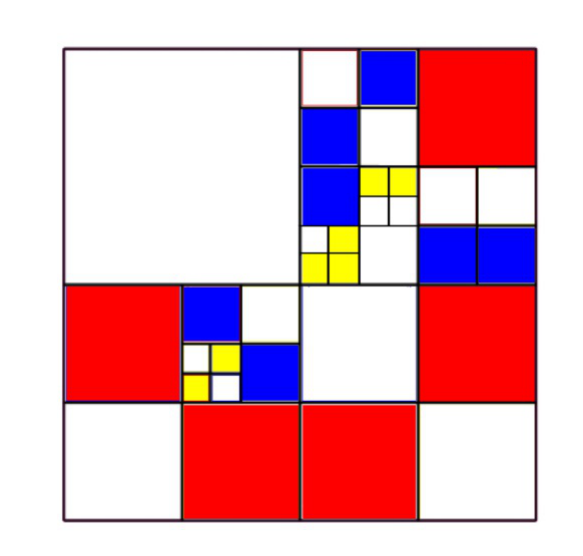
\includegraphics[width=0.35\textwidth]{figs/fig-2-1.png}
\caption{二进 Mondrian 图.}
\label{fig:2.1}
\end{figure}

\section{Vitali 覆盖}

设 $\mathcal{B}$ 是有限测度可测子集构成的族.

\begin{definition}\label{def:2.4}
族 $\mathcal{B}$ 具有 Vitali 覆盖性质 $\mathrm{V}_q$（$1 \leq q \leq \infty$）, 若存在有限常数 $C$, 使得对每一族 $\{R_i\}_{i \in I} \subset \mathcal{B}$, 都能找到子列 $\{\tilde{R}_k\}_{k \geq 1} \subset \{R_i\}_{i \in I}$, 满足下列条件:
\begin{align*}
  \mu\Big(\bigcup_{i\in I}R_{i}\Big)\leq C\,\mu\Big(\bigcup_{k}\tilde{R}_{k}\Big),
\end{align*}
\begin{align*}
  \Big\|\sum_{k}\chi_{\tilde{R}_{k}}\Big\|_{q}\leq C\,\mu\Big(\bigcup_{i\in I}R_{i}\Big)^{1/q}.
\end{align*}
这里我们使用了集合 $A$ 的示性函数的标准记号 $\chi_{A}$. 为简化表述, 且在不致混淆时, 我们将使用记号 $A(x) = \chi_{A}(x)$ 代替.
\end{definition}

\begin{theorem}\label{thm:2.5}
极大算子 $M$ 是弱型 $(p,p)$ 的, 当且仅当 $\mathcal{B}$ 满足覆盖性质 $\mathrm{V}_{q}$, 其中 $1/p+1/q=1$, $1<p<\infty$.
\end{theorem}

\begin{proof}
首先假设 $\mathcal{B}$ 具有性质 $\mathrm{V}_q$. 对 $\alpha > 0$, 令 $F_\alpha = \{x : M f(x) \geq \alpha\}$. 显然
\begin{align*}
  F_{\alpha}=\bigcup_{i\in I}R_{i},\qquad R_{i}\in\mathcal{B},
\end{align*}
且
\begin{align*}
  \frac{1}{\mu(R_{i})}\int_{R_{i}}\left|f(y)\right|\,\mathrm{d}\mu(y)>\alpha.
\end{align*}
按 $\mathrm{V}_q$ 定义选取 $\{\tilde{R}_k\}$. 则
\begin{align*}
  \mu(F_{\alpha})
  &=\mu\Big(\bigcup_{i} R_{i}\Big)\leq C\sum_{k}\mu(\tilde{R}_{k})
  \leq\frac{C}{\alpha}\sum_{k}\int_{\tilde{R}_{k}}|f(u)|\,\mathrm{d}\mu(u)\\
  &=\frac{C}{\alpha}\int\Big[\sum_{k}\tilde{R}_{k}(y)\Big]|f(y)|\,\mathrm{d}\mu(y)
  \leq\frac{C}{\alpha}\Big\|\sum_{k}\tilde{R}_{k}\Big\|_{q}\|f\|_{p}
  \leq\frac{C^{2}}{\alpha}\,\mu(F_{\alpha})^{1/q}\|f\|_{p},
\end{align*}
回忆 $1/p + 1/q = 1$, 由此得
\begin{align*}
  \mu(F_{\alpha})\leq C^{2p}\frac{\|f\|_{p}^{p}}{\alpha^{p}},
\end{align*}
即 $M$ 是弱型 $(p, p)$ 的.

反之, 设 $M$ 从 $L^p$ 到 Lorentz 空间 $L(p, \infty)$ 有界, 等价地, $M$ 是弱型 $(p, p)$ 的（\cite{b14} 含有本证明所需的 Lorentz 空间性质）. 给定陈述中的族 $\{R_i\}$, 假设存在子列 $\{\tilde{R}_k\}$, 满足 $\mu\bigl(\bigcup_i R_i\bigr) \leq C\,\mu\bigl(\bigcup_k \tilde{R}_k\bigr)$ 及下述\termcn{稀疏性}性质:
\begin{equation}\label{eq:2.3}
  \mu\Big\{\tilde{R}_{k}\cap\Big(\bigcup_{j<k}\tilde{R}_{j}\Big)\Big\}\leq\frac{1}{2}\,\mu(\tilde{R}_{k}),\quad k=1,2,\ldots.
\end{equation}
那么我们断言, 序列 $\{\tilde{R}_k\}$ 还满足 $\bigl\|\sum_k \tilde{R}_k\bigr\|_q \leq C\bigl(\bigcup_i R_i\bigr)^{1/q}$, 其中 $C < \infty$ 是某个普适常数. 为看出这一点, 令
\begin{align*}
  E_{k}=\tilde{R}_{k}\setminus\bigcup_{j<k}\tilde{R}_{j},
\end{align*}
定义线性算子
\begin{align*}
  T f(x)=\sum_{k}\left\{\frac{1}{\mu(\tilde{R}_{k})}\int_{\tilde{R}_{k}}f(y)\,\mathrm{d}\mu(y)\right\}\cdot\chi_{E_{k}}(x),
\end{align*}
并注意其伴随由下式给出:
\begin{align*}
  T^{*}f(x)=\sum_{k}\left\{\frac{1}{\mu(\tilde{R}_{k})}\int_{E_{k}}f(y)\,\mathrm{d}\mu(y)\right\}\cdot\chi_{\tilde{R}_{k}}(x).
\end{align*}
还要注意 $|Tf(x)| \leq Mf(x)$, 以及
\begin{align*}
  T^{*}\bigl(\chi_{\bigcup_{k}\tilde{R}_{k}}\bigr)(x)\geq\frac{1}{4}\sum_{k}\chi_{\tilde{R}_{k}}(x).
\end{align*}
由于（按假设）$M$ 从 $L^p$ 到 $L(p, \infty)$ 有界, 同样的结论对 $T$ 成立, 且界与 $\{\tilde{R}_k\}$ 无关. 由\newterm{duality}{对偶}{duality}, 算子 $T^*$ 必从 Lorentz 空间 $L(q,1)$ 到 $L^{q}$ 有界, 这蕴含
\begin{align*}
  \Big\|\sum_{k}\chi_{\tilde{R}_{k}}\Big\|_{q}\leq C\,\mu\Big(\bigcup_{k}\tilde{R}_{k}\Big)^{1/q},
\end{align*}
其中 $C$ 是依赖于 $M$ 的界、但不依赖于族 $\{R_{i}\}$ 的常数.

为结束证明, 必须说明如何选取具有稀疏性性质 \eqref{eq:2.3} 的序列 $\{R_k\}$. 首先, 不失一般性可设 $\{R_i\}$ 是序列 $\{R_1, R_2, \ldots\}$. 然后取 $\tilde{R}_1 = R_1$；假设已选定 $\tilde{R}_1, \ldots, \tilde{R}_k$, 取 $\tilde{R}_{k+1}$ 为序列 $\{R_i\}$ 中位于 $\tilde{R}_k$ 之后、具有性质
\begin{align*}
  \mu\Big(\tilde{R}_{k+1}\cap\Big(\bigcup_{j\leq k}\tilde{R}_{j}\Big)\Big)\leq\frac{1}{2}\,\mu(\tilde{R}_{k})
\end{align*}
的第一个元素, 并注意
\begin{align*}
  \bigcup_{j}R_{j}\subset\left\{x:M\bigl(\chi_{\bigcup_{k}\tilde{R}_{k}}\bigr)(x)\geq 1/2\right\}.
\end{align*}
\end{proof}

\begin{remark}\label{rem:2.6}
情形 $p = 1$, $q = \infty$ 不能加入定理的陈述, 因为两个蕴涵中只有一个成立. 即性质 $V_{\infty}$ 蕴含弱型 $(1, 1)$, 但反方向一般不成立. 然而, 极大函数的弱型 $(1, 1)$ 性质蕴含估计
\begin{align*}
  \int_{\bigcup_{k}R_{k}}\exp\Big(\sum_{k}\chi_{R_{k}}(x)\Big)\,\mathrm{d}\mu(x)\leq C\,\mu\Big(\bigcup_{k}R_{k}\Big)
\end{align*}
对每个满足稀疏性性质 \eqref{eq:2.3} 的序列 $\{R_{k}\}$ 成立.

一般地, 若 $M$ 从 $L(\log^{+}L)^{r}$ 到弱 $L^{1}$ 有界, 则满足稀疏性性质 \eqref{eq:2.3} 的序列必满足
\begin{equation}\label{eq:2.4}
  \int_{\bigcup_{k}R_{k}}\exp\Big(\sum_{k}\chi_{R_{k}}(x)\Big)^{1/(r+1)}\,\mathrm{d}\mu(x)\leq C\,\mu\Big(\bigcup_{k}R_{k}\Big).
\end{equation}
但这样的覆盖引理不足以保证极大函数算子从 $L(\log^{+}L)^{r}$ 到弱 $L^{1}$ 的有界性.

不等式 \eqref{eq:2.4} 的证明可以容易地由 Marcinkiewicz\newterm{interpolation}{插值}{interpolation}定理得到, 只需跟踪 $p \to 1$ 时 Hardy--Littlewood 极大函数在 $L^p(\R^n)$ 中估计常数的增长.
\end{remark}

\section{强极大函数}

现在考虑 $\R^n$ 上的 Lebesgue 测度以及各边平行于坐标轴的平行多面体（矩形）构成的族 $\mathcal{B}_n$. 再次得到相伴的极大函数 $M_n$, 对其所谓的强极大定理可以用两种等价形式陈述:

\begin{enumerate}
\item[(a)] 定量版本: $M_n$ 从 Orlicz 空间 $L(\log^+L)^{n-1}(\mathcal{Q})$ 到弱 $L^1(\mathcal{Q})$ 有界, 其中 $\mathcal{Q}$ 是 $\R^n$ 中的单位方体: 对 $\alpha > 0$,
\begin{align*}
  \mu\{M_{n}f(x)>\alpha\}\leq C_{n}\int_{\mathcal{Q}}\frac{|f(x)|}{\alpha}\Big\{1+\Big(\log^{+}\frac{|f(x)|}{\alpha}\Big)^{n-1}\Big\}\,\mathrm{d}\mu(x),
\end{align*}
其中 $C_{n}$ 是仅依赖于维数 $n$ 的常数；

\item[(b)] 定性版本: 基 $\mathcal{B}_n$ 微分属于空间 $L(\log^+ L)^{n-1}$ 的局部函数的积分, 即
\begin{align*}
  \lim_{\substack{x\in R\\ \mathrm{diam}(R)\to 0}}\frac{1}{\mu(R)}\int_{R}f(y)\,\mathrm{d}\mu(y)=f(x),\quad\text{a.e.}\ x\in\R^{n},
\end{align*}
对每个局部属于 $L(\log^{+}L)^{n-1}(\R^{n})$ 的函数 $f$ 成立.
\end{enumerate}

\newterm{strong-maximal-function}{强极大函数}{strong maximal function}在与多参数膨胀族交换的算子的研究中颇为要紧, 在这里参数的数目至关重要, 它改变结果的性质.

例如, 当 $n \geq 2$ 时, $M_n$ 不满足 Hardy--Littlewood 不等式. 例如, 当 $n = 2$ 时取
\begin{align*}
  f_{\varepsilon}(x_{1},x_{2})=\frac{1}{\varepsilon^{2}}\,\chi_{\{|x_{1}|<\varepsilon/2,\ |x_{2}|<\varepsilon/2\}},
\end{align*}
则对 $|x_1|, |x_2| > 2\varepsilon$, 有 $M_2f_\varepsilon(x_1, x_2) \sim 1/(|x_1|\,|x_2|)$.

设 $Q_{0} = [-1, 1] \times [-1, 1]$. 则
\begin{align*}
  \mu\{x\in Q_{0}:M_{2}f_{\varepsilon}>\lambda\}
  \geq\mu\{x\in Q_{0}:|x_{1}\cdot x_{2}|<1/\lambda\}
  \sim\frac{1}{\lambda}\left|\log\frac{1}{\lambda}\right|,\quad\text{若 } \lambda=1/\varepsilon,
\end{align*}
而我们想要的是与 Hardy--Littlewood 极大函数所满足者类似的不等式. 由此可知 $\|f_\varepsilon\| \geq c\log\frac{1}{\varepsilon}$, 而使其成立的最小 Orlicz 范数正是 $L(\log^+ L)$ 范数.

上面引述的结果 (a) 与 (b) 归功于 Jessen、Marcinkiewicz 与 Zygmund \cite{b57}. 其证明的主要思想是用复合 $M_{x_1} \cdot M_{x_2} \cdots M_{x_n}$ 来控制算子 $M_n$, 其中 $M_{x_j}$ 表示沿第 $j$ 个坐标轴方向的一维 Hardy--Littlewood 极大算子. 该论证的优雅与简洁是显然的. 然而, 似乎宜于有一个基于恰当覆盖引理的几何证明. 主要原因是, 对别的测度我们缺乏乘积结构, 而获得与强极大函数类似算子的结果的唯一途径, 是通过对\newterm{rectangle}{矩形}{rectangle}几何的深刻理解.

图~\ref{fig:2.2} 表明 Vitali 覆盖引理对 $\R^n$（$n \geq 2$）中的平行多面体不成立. 注意 $\mu(R_1) = \mu(R_2) = \cdots = \mu(R_k) = 1$. 矩形序列 $\{R_k\}$ 满足性质 \eqref{eq:2.3}, 但没有任何办法选出满足 Vitali 覆盖要求的子族.

\begin{figure}[htbp]
\centering
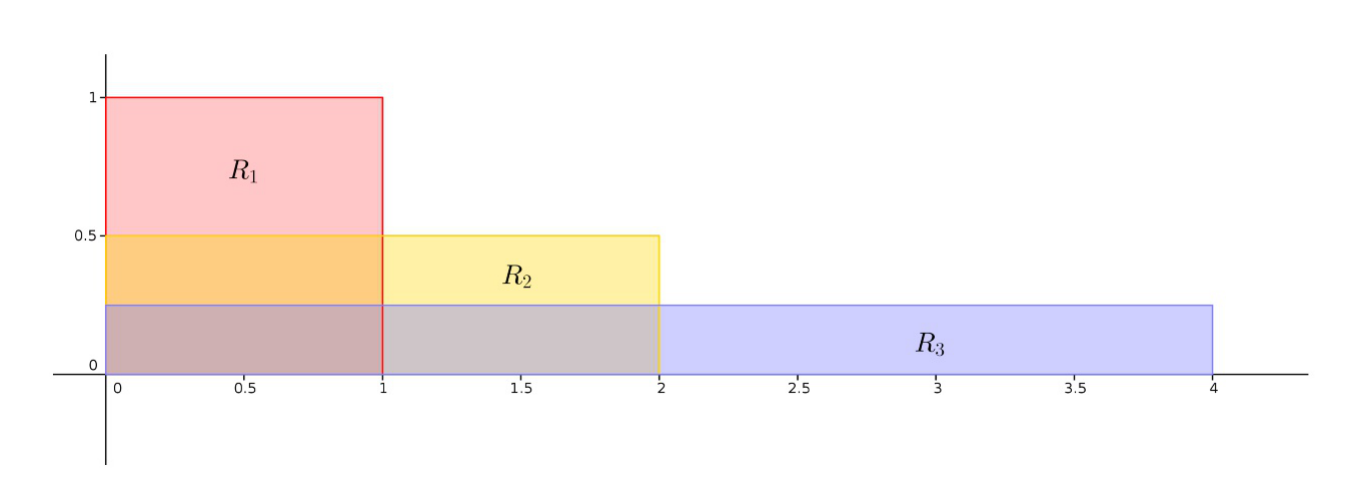
\includegraphics[width=0.72\textwidth]{figs/fig-2-2.png}
\caption{Vitali 覆盖引理对平行多面体不成立.}
\label{fig:2.2}
\end{figure}

\begin{theorem}\label{thm:2.7}
设 $\{R_k\}$ 是 $\R^n$ 中一列各边平行于坐标轴的平行多面体, 其并集有界. 则存在子列 $\{\tilde{R}_j\} \subset \{R_k\}$, 使得
\begin{enumerate}
\item[(1)] $\mu\Big(\bigcup_{k}R_{k}\Big)\leq C_{n}\,\mu\Big(\bigcup_{j}\tilde{R}_{j}\Big)$；
\item[(2)] $\Big\|\exp\Big(\sum_{j}\chi_{\tilde{R}_j}\Big)^{1/(n-1)}-1\Big\|_1 \leq C_n\,\mu\Big(\bigcup_j \tilde{R}_j\Big)$, 其中 $C_n < \infty$ 是普适常数.
\end{enumerate}
\end{theorem}

在证明这一定理之前, 让我们说明它蕴含上述 Jessen、Marcinkiewicz 与 Zygmund 的结果. 设 $\alpha > 0$. 对每个点 $x \in \{M_n f(x) > \alpha\}$, 存在含 $x$ 的矩形 $R_x$, 满足
\begin{align*}
  \frac{1}{\left|R_{x}\right|}\int_{R_{x}}\left|f\right|>\alpha.
\end{align*}
不失一般性, 假设 $\bigcup_x R_x = \bigcup_k R_k$, 其中 $R_k$ 是某些 $R_x$. 应用覆盖引理得到满足定理 2.7 中性质 (1) 与 (2) 的 $\tilde{R}_k$. 于是由 (1), 只须证明
\begin{align*}
  \mu\Big(\bigcup_{k}\tilde{R}_{k}\Big)\leq C_{n}\int_{\R^{n}}\frac{|f(x)|}{\alpha}\log^{n-1}\left(1+\frac{|f(x)|}{\alpha}\right)\mathrm{d}x.
\end{align*}
由于 $\mu(R_k) \leq \frac{1}{\alpha} \int_{R_k} |f|$, 求和得
\begin{align*}
  \mu\Big(\bigcup_{k}\tilde{R}_{k}\Big)\leq\frac{1}{\alpha}\int_{Q_{0}}|f|\sum_{k}\chi_{\tilde{R}_{k}}.
\end{align*}
适当应用 Young 不等式 $ab \leq e^a - b + b\log b$（$a, b > 0$）, 即得结果.

\begin{proof}[定理~\ref{thm:2.7} 的证明]
我们对 $n$ 作归纳. 假设 $n-1$ 的情形, 并把 $R_1, R_2, \ldots$ 排列成 $x_n$ 方向边长递减的顺序. 对矩形 $R$, 用 $R_d$ 表示与 $R$ 同心、对 $i < n$ 各 $x_i$ 方向边长相同、但 $x_n$ 方向边长乘以 $5$ 的矩形. 下面描述从 $R_k$ 中选取 $\tilde{R}_k$ 的程序. 令 $\tilde{R}_1 = R_1$. 假设 $\tilde{R}_1, \tilde{R}_2, \ldots, \tilde{R}_k$ 已经选定. 我们继续沿列表前行, 每次考虑矩形 $R$ 时, 询问是否
\begin{align*}
  \mu\Big(R\cap\Big(\bigcup_{j}(\tilde{R}_{j})_{d}\Big)\Big)<\frac{1}{2}\,\mu(R),
\end{align*}
其中上面的并取遍满足 $\tilde{R}_j \cap R \neq \emptyset$ 的一切 $j \leq k$. 若答案是否定的, 就移到列表的下一个矩形. 若答案是肯定的, 就把这个矩形 $R$ 定为 $\tilde{R}_{k+1}$, 并重新开始这一过程.

现在如下证明 (1). 若 $R$ 是未被选中的矩形, 则
\begin{align*}
  \mu\Biggl(R\cap\Big[\bigcup_{\substack{\tilde{R}_{j}\cap R\neq\emptyset\\ \tilde{R}_{j}\ \text{在}\ R\ \text{之前}}}(\tilde{R}_{j})_{d}\Big]\Biggr)\geq\frac{1}{2}\,\mu(R).
\end{align*}
用垂直于 $x_n$ 轴的超平面把所有矩形切片. 若切片用 $S$ 代替 $R$ 表示, 则
\begin{align*}
  \mu\Big(S\cap\Big(\bigcup_{j}(\tilde{S}_{j})_{d}\Big)\Big)\geq\frac{1}{2}\,\mu(S),
\end{align*}
从而在 $\bigcup_{j}R_{j}$ 上有
\begin{align*}
  M_{n-1}\bigl(\chi_{\bigcup_{j}(\tilde{R}_{j})_{d}}\bigr)>1/2,
\end{align*}
其中 $M_{n-1}$ 作用于 $x_1, x_2, \ldots, x_{n-1}$ 坐标.

由 $M_{n-1}$ 在（比如）$L^2$ 上的有界性（归纳假设）, 得
\begin{align*}
  \mu\Big(\bigcup_{j}R_{j}\Big)\leq C\,\mu\Big(\bigcup_{k}(\tilde{R}_{k})_{d}\Big)
  \leq C^{\prime}\sum_{k}\mu(\tilde{R}_{k})
  \leq C^{\prime}\,\mu\Big(\bigcup_{k}\tilde{R}_{k}\Big).
\end{align*}

为得到 (2), 注意诸 $\tilde{R}_{j}$ 满足
\begin{align*}
  \mu\Biggl(\tilde{R}_{k}\cap\Big[\bigcup_{\substack{\tilde{R}_{j}\cap\tilde{R}_{k}\neq\emptyset\\ j<k}}(\tilde{R}_{j})_{d}\Big]\Biggr)<\frac{1}{2}\,\mu(\tilde{R}_{k}).
\end{align*}
再用垂直于 $x_{n}$ 轴的超平面切片, 得到
\begin{align*}
  \mu\Big(\tilde{S}_{k}\cap\Big(\bigcup_{j<k}\tilde{S}_{j}\Big)\Big)<\frac{1}{2}\,\mu(\tilde{S}_{k}),
\end{align*}
故若令
\begin{align*}
  \widetilde{E}_{k}=\widetilde{S}_{k}\setminus\bigcup_{j<k}\widetilde{S}_{j},
\end{align*}
则有 $\mu(\widetilde{E}_k) > \frac{1}{2}\,\mu(\widetilde{S}_k)$；且若 $\phi \in L(\log L)^{n-1}(S_0)$, 我们将证明
\begin{equation}\label{eq:2.5}
  \int_{S_{0}}\sum_{k}\chi_{\tilde{S}_{k}}\,\phi\leq C\left\|\phi\right\|_{L(\log L)^{n-1}},
\end{equation}
由此得到
\begin{align*}
  \int_{S_{0}}\exp\left[c\Big(\sum_{k}\chi_{\tilde{S}_{k}}\Big)^{1/(n-1)}\right]\mathrm{d}x_{1}\cdots\mathrm{d}x_{n-1}\leq C.
\end{align*}
把这个估计对 $x_{n}$ 积分即可结束.

为得到 \eqref{eq:2.5}, 我们写
\begin{align*}
  \int_{S_{0}}\sum_{k}\chi_{\tilde{S}_{k}}\,\phi\;\mathrm{d}x_{1}\cdots\mathrm{d}x_{n-1}
  &\leq\sum_{k}\int_{\tilde{S}_{k}}\phi
  \leq C\sum_{k}|\widetilde{E}_{k}|\,\frac{1}{|\tilde{S}_{k}|}\int_{\tilde{S}_{k}}\phi\\
  &\leq C\int_{S_{0}}M_{n-1}(\phi)\;\mathrm{d}x_{1}\mathrm{d}x_{2}\cdots\mathrm{d}x_{n-1}
  \leq C^{\prime}\|\phi\|_{L(\log L)^{n-1}}.
\end{align*}

在上述论证中, 切片是最重要的思想. 若不切片而直接尝试证明, 我们得到的将不是 $\exp(\cdot)^{1/(n-1)}$ 范数上的估计, 而是 $\exp(\cdot)^{1/n}$ 范数上的估计. 而且, 切片正是我们用以用较低参数算子 $M_{n-1}$ 控制 $M_n$ 的机制, 这使我们能够进行归纳.
\end{proof}

\begin{figure}[htbp]
\centering
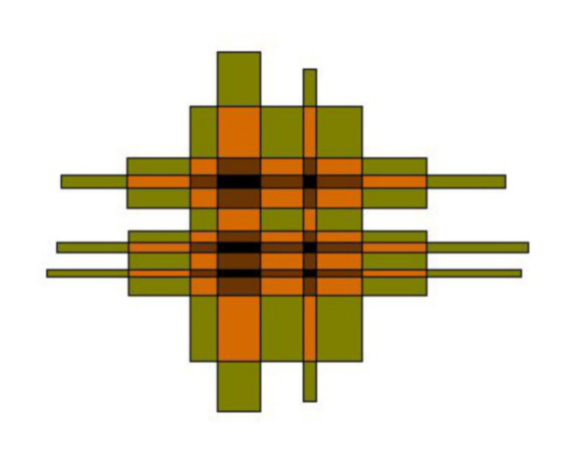
\includegraphics[width=0.42\textwidth]{figs/fig-2-3.png}
\caption{指数重叠.}
\label{fig:2.3}
\end{figure}

\section{A. Zygmund 的一个问题}

设 $\phi$ 是 $\R^2$ 中一个对每个变量分别单调的正函数. 考虑族 $\mathcal{B}_\phi = \mathcal{B}_2 \times \phi$, 即各边垂直于坐标轴、尺寸为 $s \times t \times \phi(s, t)$（$s$、$t$ 为正实数）的平行多面体. 注意, 强极大定理断言: 由于 $\mathcal{B}_\phi \subset \mathcal{B}_3$, 它微分局部属于 $L(\log^{+}L)^2(\R^3)$ 的函数的积分.

然而, 由于族 $\mathcal{B}_{\phi}$ 的平行多面体的竖直方向受限于某个单调函数的图象, 我们可以指望得到一些额外的正则性, 但要记住, 我们不可能得到比 $\mathcal{B}_2$ 更好的微分性质. 事实上, 我们将证明最优的可能改进已经达到. 让我们用两种等价形式陈述结果.

\begin{theorem}\label{thm:2.8}
\begin{enumerate}
\item[(1)] 平行多面体族 $\mathcal{B}_\phi$ 微分局部属于 $L(\log^+L)(\R^3)$ 的函数的积分, 即
\begin{align*}
  \lim_{R\to x}\frac{1}{\mu(R)}\int_{R} f(y)\,\mathrm{d}\mu(y)=f(x),\quad\text{a.e.}\ x,
\end{align*}
只要 $f \in L(\log^{+}L)(\R^{3})$, 其中 $\mu$ 表示 $\R^{3}$ 中的 Lebesgue 测度.

\item[(2)] 相伴的极大函数
\begin{align*}
  M_{\phi}f(x)=\sup_{R\ni x}\frac{1}{\mu(R)}\int_{R}\left|f(y)\right|\,\mathrm{d}\mu(y)
\end{align*}
满足不等式
\begin{align*}
  \mu\{x:M_{\phi}f(x)>\lambda\}\leq C\int\frac{|f(y)|}{\lambda}\left(1+\log^{+}\frac{|f(y)|}{\lambda}\right)\mathrm{d}\mu(y),
\end{align*}
其中 $C < \infty$ 是某个普适常数.
\end{enumerate}
\end{theorem}

为证明这一结果, 我们将再一次为族 $\mathcal{B}_{\phi}$ 发展一个合适的覆盖引理. 先引入一个定义.

\begin{definition}\label{def:2.9}
称 $\R^3$ 中平行多面体的族 $\mathcal{B}$ 是单调的, 若给定尺寸分别为 $s_1 \times t_1 \times u_1$ 与 $s_2 \times t_2 \times u_2$ 的任意两个平行多面体 $R_1$ 与 $R_2$, 下列蕴涵成立: 若 $s_1 < s_2$ 且 $t_1 < t_2$, 则 $u_1 \leq u_2$.
\end{definition}

为简化直觉与计算, 我们将局限于单调族 $\mathcal{B}$ 的平行多面体为\newterm{dyadic}{二进的}{dyadic}的情形. 下面的覆盖引理将蕴含定理 2.8.

\begin{lemma}\label{lem:2.10}
设 $\mathcal{B}$ 是 $\R^3$ 中单调的二进平行多面体族. 对满足 $\mu\bigl(\bigcup_{i\in I} R_i\bigr) < \infty$ 的每一族 $\{R_i\}_{i\in I} \subset \mathcal{B}$, 都能找到有限子列 $\{\tilde{R}_j\}_{j=1}^M \subset \{R_i\}_{i\in I}$, 同时满足
\begin{align*}
  \mu\Big(\bigcup_{i\in I}R_{i}\Big)\leq C\,\mu\Big(\bigcup_{j=1}^{M}\tilde{R}_{j}\Big),
\end{align*}
\begin{align*}
  \int_{\bigcup_{j=1}^{M}\tilde{R}_{j}}\exp\Big(\sum_{j=1}^{M}\chi_{\tilde{R}_{j}}(x)\Big)\,\mathrm{d}\mu(x)
  \leq C\,\mu\Big(\bigcup_{j=1}^{M}\tilde{R}_{j}\Big),
\end{align*}
其中 $C < \infty$ 是普适常数.
\end{lemma}

\begin{proof}
首先注意, 由于 $\mu\bigl(\bigcup_i R_i\bigr) < \infty$, 不失一般性可设 $\{R_i\}_{i \in I}$ 是有限序列 $\{R_i\}_{i=1}^N$, 使得
\begin{align*}
  \mu\Big(R_{i}\cap\Big(\bigcup_{j\neq i}R_{j}\Big)\Big)\leq\frac{1}{2}\,\mu(R_{i}),\quad i=1,\ldots,N.
\end{align*}
此外, 把序列重新排列, 使平行多面体的 $x_3$ 方向尺寸 $d_3(R_i)$ 递减, 即
\begin{align*}
  d_{3}(R_{k})\geq d_{3}(R_{k+1}),\quad k=1,2,\ldots .
\end{align*}
我们以选取 $\tilde{R}_1 = R_1$ 开始选择过程. 然后取 $\tilde{R}_k$ 为序列中满足
\begin{equation}\label{eq:2.6}
  \int_{\tilde{R}_{k}}\exp\Big(\sum_{j=1}^{k-1}\tilde{R}_{j}(x)\Big)\,\mathrm{d}\mu(x)
  \leq(1+e^{-1})\,\mu(\tilde{R}_{k})
\end{equation}
的下一个元素. 注意, $e^{-1}$ 可以换成某个别的适当常数. 下面将证明序列 $\{\tilde{R}_k\}_{k=1}^M$ 满足性质 (2):
\begin{align*}
  \int_{\bigcup_{j=1}^{M}\widetilde{R}_{j}}&\exp\left(\sum_{j=1}^{M}\chi_{\widetilde{R}_{j}}(x)\right)\mathrm{d}\mu(x)\\
  &=\int_{\bigcup_{j=1}^{M-1}\widetilde{R}_{j}\setminus\widetilde{R}_{M}}\exp\left(\sum_{j=1}^{M-1}\chi_{\widetilde{R}_{j}}(x)\right)\mathrm{d}\mu(x)
   +\int_{\widetilde{R}_{M}}\exp\left(\sum_{j=1}^{M}\chi_{\widetilde{R}_{j}}(x)\right)\mathrm{d}\mu(x)\\
  &=\int_{\bigcup_{j=1}^{M-1}\widetilde{R}_{j}\setminus\widetilde{R}_{M}}\exp\left(\sum_{j=1}^{M-1}\chi_{\widetilde{R}_{j}}(x)\right)\mathrm{d}\mu(x)
   +e\int_{\widetilde{R}_{M}}\exp\left(\sum_{j=1}^{M-1}\chi_{\widetilde{R}_{j}}(x)\right)\mathrm{d}\mu(x).
\end{align*}
但根据我们的选取 \eqref{eq:2.6}, 第二个积分项可以被控制, 于是得
\begin{align*}
  \int_{\bigcup_{j=1}^{M}\tilde{R}_{j}}\exp\Big(&\sum_{j=1}^{M}\chi_{\tilde{R}_{j}}(x)\Big)\mathrm{d}\mu(x)\\
  &\leq\int_{\bigcup_{j=1}^{M-1}\tilde{R}_{j}}\exp\Big(\sum_{j=1}^{M-1}\chi_{\tilde{R}_{j}}(x)\Big)\mathrm{d}\mu(x)+(1+e)\,\mu(\tilde{R}_{M}).
\end{align*}
迭代这一过程, 得到如下控制:
\begin{align*}
  \int_{\bigcup_{j=1}^{M}\tilde{R}_{j}}\exp\Big(\sum_{j=1}^{M}\chi_{\tilde{R}_{j}}(x)\Big)\mathrm{d}\mu(x)
  \leq(1+e)\sum_{k=1}^{M}\mu(\tilde{R}_{k})
  \leq 2(1+e)\,\mu\Big(\bigcup_{k=1}^{M}\tilde{R}_{k}\Big).
\end{align*}

我们的目标现在是证明我们没有丢弃``太多''平行多面体, 即
\begin{align*}
  \mu\Big(\bigcup_{i=1}^{N} R_{i}\Big)\leq C\,\mu\Big(\bigcup_{j=1}^{M}\tilde{R}_{j}\Big).
\end{align*}
设 $R$ 是被丢弃的平行多面体. 则由于族 $\{\tilde{R}_j\}_{j=1}^M$ 已经按竖直尺寸 $d_3(\tilde{R}_j)$ 递减排列, 必有
\begin{align*}
  1+e^{-1}<\frac{1}{\mu(R)}\int_{R}\exp\Big(\sum_{d_{3}(\tilde{R}_{j})\geq d_{3}(R)}\chi_{\tilde{R}_{j}}(x)\Big)\mathrm{d}\mu(x).
\end{align*}
注意, 由于族 $\mathcal{B}_\phi$ 是单调的, 若 $d_3(\tilde{R}_j) \geq d_3(R)$, 则必有
\begin{align*}
  d_{1}(\tilde{R}_{j})\geq d_{1}(R)\quad\text{或}\quad d_{2}(\tilde{R}_{j})\geq d_{2}(R).
\end{align*}
于是可以把上面的不等式改写成
\begin{equation}\label{eq:2.7}
  \begin{aligned}
  1+e^{-1}&<\frac{1}{\mu(R)}\int_{R}\exp\left(\sum_{\substack{d_{3}(\tilde{R}_{j})\geq d_{3}(R)\\ d_{1}(\tilde{R}_{j})\geq d_{1}(R)}}\chi_{\tilde{R}_{j}}(x)\right)
   \cdot\exp\left(\sum_{\substack{d_{3}(\tilde{R}_{j})\geq d_{3}(R)\\ d_{2}(\tilde{R}_{j})\geq d_{2}(R)}}\chi_{\tilde{R}_{j}}(x)\right)\mathrm{d}\mu(x)\\
  &=\frac{1}{\mu(R)}\int_{R}\exp\left(\sum_{i=1}^{k}\chi_{\tilde{R}_{\nu_{i}}}(x)\right)
   \cdot\exp\left(\sum_{j=1}^{l}\chi_{\tilde{R}_{\mu_{j}}}(x)\right)\mathrm{d}\mu(x),
  \end{aligned}
\end{equation}
其中 $\tilde{R}_{\nu_1}, \ldots, \tilde{R}_{\nu_k}$ 是第一个和中的平行多面体, $\tilde{R}_{\mu_1}, \ldots, \tilde{R}_{\mu_l}$ 是第二个和中的那些.

固定平行多面体 $R$, 不失一般性, 可简化记号, 改换指标使得对 $i = 1, \ldots, k$ 有 $\tilde{R}_{\nu_i} = \tilde{R}_i$, 对 $j = 1, \ldots, l$ 有 $\tilde{R}_{\mu_j} = \tilde{R}_{k+j}$. 现在把积分号内的指数展开:
\begin{align*}
  \exp\Big(\sum_{i=1}^{k}\chi_{\tilde{R}_{\nu_{i}}}(x)\Big)
  &=\sum_{n=0}^{\infty}\frac{1}{n!}\Big(\sum_{i=1}^{k}\chi_{\tilde{R}_{\nu_{i}}}(x)\Big)^{n}
  =\sum_{n=0}^{\infty}\frac{1}{n!}\sum_{i_{1},\ldots,i_{n}=1}^{k}
   \chi_{\tilde{R}_{i_{1}}}(x)\cdots\chi_{\tilde{R}_{i_{n}}}(x),\\
  \exp\Big(\sum_{j=1}^{l}\chi_{\tilde{R}_{\mu_{j}}}(x)\Big)
  &=\sum_{m=0}^{\infty}\frac{1}{m!}\Big(\sum_{j=1}^{l}\chi_{\tilde{R}_{\mu_{j}}}(x)\Big)^{m}
  =\sum_{m=0}^{\infty}\frac{1}{m!}\sum_{j_{1},\ldots,j_{m}=k+1}^{k+l}
   \chi_{\tilde{R}_{j_{1}}}(x)\cdots\chi_{\tilde{R}_{j_{m}}}(x).
\end{align*}
最后这些和式项正是 $n$ 个因子 $\chi_{\tilde{R}_{\nu_{i}}}$（或分别地, $m$ 个因子 $\chi_{\tilde{R}_{\mu_{i}}}$）乘积的所有可能组合. 因此, 把这个表达式用于 \eqref{eq:2.7}, 得到
\begin{align*}
  \sum_{n,m=0}^{\infty}&\frac{1}{n!\,m!}\sum_{i_{1},\ldots,i_{n}=1}^{k}\sum_{j_{1},\ldots,j_{m}=k+1}^{k+l}
  \frac{1}{\mu(R)}\int_{R}\chi_{\tilde{R}_{i_{1}}}(x)\cdots\chi_{\tilde{R}_{j_{m}}}(x)\,\mathrm{d}\mu(x)\\
  &=\sum_{n,m=0}^{\infty}\frac{1}{n!\,m!}\sum_{i_{1},\ldots,i_{n}=1}^{k}\sum_{j_{1},\ldots,j_{m}=k+1}^{k+l}
  \frac{\mu\{\tilde{R}_{i_{1}}\cap\cdots\cap\tilde{R}_{i_{n}}\cap\tilde{R}_{j_{1}}\cap\cdots\cap\tilde{R}_{j_{m}}\cap R\}}{\mu(R)}.
\end{align*}

现在很清楚, 为证明性质 (1), 关键在于控制平行多面体 $\tilde{R}_{i_1}, \ldots, \tilde{R}_{j_m}$ 与 $R$ 的重叠. 注意, 若相交不空, 则交集必呈图~\ref{fig:2.4} 所示的形状. 即, 对应于 $\varepsilon$ 的块是 $\tilde{R}_{i_1}, \ldots, \tilde{R}_{i_n}$ 的交, 对应于 $\delta$ 的块是 $\tilde{R}_{j_1}, \ldots, \tilde{R}_{j_m}$ 的交. 注意这里我们使用了所处理的是二进平行多面体这一事实: 若交集不空, 则切口必须是``干净的'', 即某一边尺寸较长的平行多面体把其余者沿该边方向完全切开.

\begin{figure}[htbp]
\centering
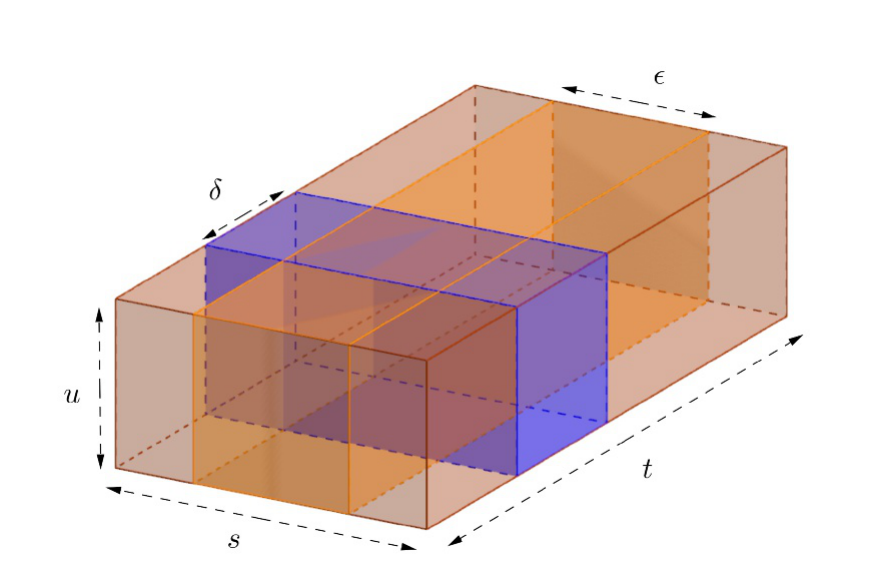
\includegraphics[width=0.45\textwidth]{figs/fig-2-4.png}
\caption{控制交集.}
\label{fig:2.4}
\end{figure}

于是交集 $\tilde{R}_{i_1} \cap \cdots \cap R_{i_n} \cap \tilde{R}_{j_1} \cap \cdots \cap \tilde{R}_{j_m}$ 将是尺寸为 $\varepsilon \times \delta \times u$ 的平行多面体. 由此得
\begin{align*}
  \frac{\mu\{\tilde{R}_{i_{1}}\cap\cdots\cap\tilde{R}_{i_{n}}\cap\tilde{R}_{j_{1}}\cap\cdots\cap\tilde{R}_{j_{m}}\cap R\}}{\mu(R)}
  =\frac{\varepsilon\times\delta}{s\times t},
\end{align*}
并且有
\begin{equation}\label{eq:2.8}
  1+e^{-1}<\sum_{n,m=0}^{\infty}\frac{1}{n!\,m!}\sum_{i_{1},\ldots,i_{n}=1}^{k}\sum_{j_{1},\ldots,j_{m}=k+1}^{k+l}\frac{\varepsilon\times\delta}{s\times t}.
\end{equation}

接下来更仔细地考察所有这些平行多面体的交集. 这次固定交集内的一点 $P = (x_0, y_0, z_0)$, 考虑与 $R$ 相交的水平平面与竖直平面（见图~\ref{fig:2.5}）以及线段
\begin{align*}
  I_{P}^{1}=\{\left(x,y_{0},z_{0}\right)\in R\},\qquad
  I_{P}^{2}=\{\left(x_{0},y,z_{0}\right)\in R\}.
\end{align*}

\begin{figure}[htbp]
\centering
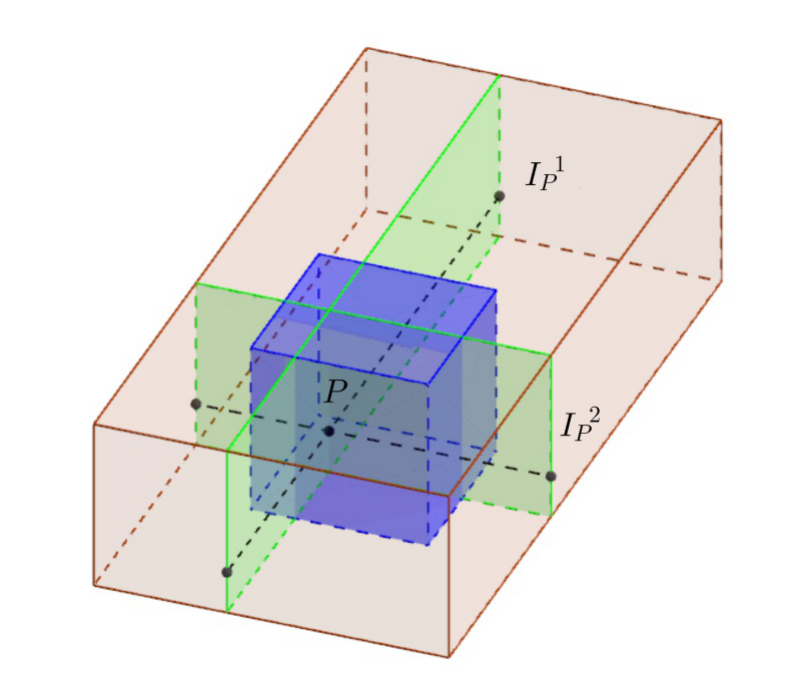
\includegraphics[width=0.4\textwidth]{figs/fig-2-5.png}
\caption{线段 $I_{P}^{1}$ 与 $I_{P}^{2}$.}
\label{fig:2.5}
\end{figure}

由单调性, 得
\begin{align*}
  \frac{|\tilde{R}_{i_{1}}\cap\cdots\cap\tilde{R}_{i_{n}}\cap I_{P}^{1}|}{|I_{P}^{1}|}=\frac{\varepsilon}{s},\qquad
  \frac{|\tilde{R}_{j_{1}}\cap\cdots\cap\tilde{R}_{j_{m}}\cap I_{P}^{2}|}{|I_{P}^{2}|}=\frac{\delta}{t}.
\end{align*}
这里 $|\cdot|$ 指一维 Lebesgue 测度. 把这两个量之积代入 \eqref{eq:2.8}, 得到方向 Hardy--Littlewood 极大函数的一个下界:
\begin{align*}
  1+e^{-1}
  &<\sum_{n,m=0}^{\infty}\frac{1}{n!\,m!}\sum_{i_{1},\ldots,i_{n}=1}^{k}\sum_{j_{1},\ldots,j_{m}=k+1}^{k+l}
   \frac{|\tilde{R}_{i_{1}}\cap\cdots\cap\tilde{R}_{i_{n}}\cap I_{P}^{1}|}{|I_{P}^{1}|}
   \cdot\frac{|\tilde{R}_{j_{1}}\cap\cdots\cap\tilde{R}_{j_{m}}\cap I_{P}^{2}|}{|I_{P}^{2}|},
\end{align*}
因此
\begin{align*}
  1+e^{-1}
  &<\Big\{\frac{1}{|I_{P}^{1}|}\int_{I_{P}^{1}}\exp\Big(\sum_{i=1}^{k}\chi_{\tilde{R}_{i}}(x)\Big)\mathrm{d}x\Big\}
   \cdot\Big\{\frac{1}{|I_{P}^{2}|}\int_{I_{P}^{2}}\exp\Big(\sum_{j=k+1}^{k+l}\chi_{\tilde{R}_{j}}(x)\Big)\mathrm{d}x\Big\}\\
  &<M_{1}\Big(\exp\Big(\sum_{i=1}^{k}\chi_{\tilde{R}_{i}}(x)\Big)\Big)(P)
   \cdot M_{2}\Big(\exp\Big(\sum_{j=k+1}^{k+l}\chi_{\tilde{R}_{j}}(x)\Big)\Big)(P),
\end{align*}
其中 $M_1$ 与 $M_2$ 分别表示沿 $x_1$ 与 $x_2$ 方向的一维 Hardy--Littlewood 极大函数到 $\R^3$ 上的扩张. 我们已证明, 对任何被丢弃的平行多面体, 有下面的包含关系:
\begin{align*}
  R&\subset\Big\{x:M_{1}\Big(\exp\Big(\sum_{i=1}^{M}\chi_{\tilde{R}_{i}}\Big)\Big)
   \cdot M_{2}\Big(\exp\Big(\sum_{j=1}^{M}\chi_{\tilde{R}_{j}}(x)\Big)\Big)>1+e^{-1}\Big\}\\
  &\subset\Big\{x:M_{1}\Big(\exp\Big(\sum_{i=1}^{M}\chi_{\tilde{R}_{i}}\Big)\Big)>\sqrt{1+e^{-1}}\Big\}
   \cup\Big\{x:M_{2}\Big(\exp\Big(\sum_{j=1}^{M}\chi_{\tilde{R}_{j}}(x)\Big)\Big)>\sqrt{1+e^{-1}}\Big\}.
\end{align*}
最后,
\begin{align*}
  \mu\Big(\bigcup_{i\in I}R_{i}\Big)
  &\leq\frac{2}{\sqrt{1+e^{-1}}}\int_{\bigcup_{j=1}^{M}\tilde{R}_{j}}\exp\Big(\sum_{j=1}^{M}\chi_{\tilde{R}_{j}}(x)\Big)\mathrm{d}\mu(x)\\
  &\leq 4\sqrt{1+e^{-1}}\;\mu\Big(\bigcup_{j=1}^{M}\tilde{R}_{j}\Big).
\end{align*}
\end{proof}

\begin{proof}[定理~\ref{thm:2.8} 的证明]
众所周知 (1) 与 (2) 是等价的, 其中蕴涵 (2) $\Rightarrow$ (1) 是较容易的一个. 证明的策略如下: 首先观察到, 若族 $\mathcal{B}$ 满足覆盖引理的假设, $M$ 表示与 $\mathcal{B}$ 相伴的极大函数, 则 $M$ 满足 (2). 接着, 我们找到具有性质 $M_{\phi}f \leq CMf$（$C$ 为普适常数）的这样的族 $\mathcal{B}$.

设 $\mathcal{B}$ 满足覆盖引理的假设, 定义
\begin{align*}
  M f(x)=\sup_{x\in R^{*},\;R\in\mathcal{B}}\frac{1}{\mu(R)}\int_{R}|f(y)|\,\mathrm{d}\mu(y),
\end{align*}
其中 $R^{*}$ 是把 $R$ 关于其中心以因子 $3$ 膨胀的结果.

\begin{claim*}
存在常数 $C < \infty$, 使得
\begin{align*}
  \mu(\{M f(x)>\lambda\})\leq C\int_{\R^{3}}\frac{|f(x)|}{\lambda}\left\{1+\log^{+}\frac{|f(x)|}{\lambda}\right\}\mathrm{d}\mu(x).
\end{align*}
\end{claim*}

\begin{proof}[断言的证明]
集合 $\{Mf(x) > \lambda\}$ 是满足
\begin{align*}
  \frac{1}{\mu(R_{\alpha})}\int_{R_{\alpha}}\left|f(y)\right|\,\mathrm{d}\mu(y)\geq\lambda
\end{align*}
的平行多面体 $\{R_\alpha\}$ 之并. 可以应用覆盖引理证明具有给定性质的子族 $\{R_{j}\}$ 的存在性. 我们有
\begin{align*}
  \mu\Big(\bigcup_{j}R_{j}^{*}\Big)
  \leq 27\sum_{j}\mu\Big(\bigcup_{j}R_{j}\Big)
  \leq 27\int_{\bigcup_{j}R_{j}}\frac{|f(x)|}{\lambda}\sum_{j}\chi_{R_{j}}(x)\,\mathrm{d}\mu(x).
\end{align*}
其次注意, 若 $u$ 与 $v$ 是正实数, 则 $u\cdot v \leq u\log u + e^{v-1}$. 此外, 对每个 $\varepsilon > 0$, 存在常数 $C_\varepsilon < \infty$, 使得 $u\cdot v \leq C_\varepsilon\,u(1 + \log^+ u) + e^{\varepsilon v - 1}$. 特别地,
\begin{align*}
  \mu\Big(\bigcup_{j} R_{j}^{*}\Big)
  \leq&\,C_{\varepsilon}\int_{\bigcup_{j} R_{j}}\frac{|f(x)|}{\lambda}\left\{1+\log^{+}\frac{|f(x)|}{\lambda}\right\}\mathrm{d}\mu(x)\\
  &+e^{-1}\int_{\bigcup_{j} R_{j}}\exp\Big(\varepsilon\sum_{j}\chi_{R_{j}}(x)\Big)\mathrm{d}\mu(x).
\end{align*}
但
\begin{align*}
  \int_{\bigcup_{j}R_{j}}&\exp\Big(\varepsilon\sum_{j}\chi_{R_{j}}(x)\Big)\mathrm{d}\mu(x)\\
  &\leq\Big[\mu\Big(\bigcup_{j}R_{j}\Big)\Big]^{1-\varepsilon}
   \Big(\int_{\bigcup_{j}R_{j}}\exp\Big(\sum_{j}\chi_{R_{j}}(x)\Big)\mathrm{d}\mu(x)\Big)^{\varepsilon}
  \leq C^{\varepsilon}\,\mu\Big(\bigcup_{j}R_{j}\Big),
\end{align*}
其中 $C$ 是覆盖引理中出现的常数. 为结束证明, 只需选取 $\varepsilon > 0$ 使 $C^{\varepsilon}e^{-1} \leq 1/2$.
\end{proof}

最后, 必须说明如何从 $\mathcal{B}_\phi$ 得到族 $\mathcal{B}$. 首先, 把 $s$ 与 $t$ 的值化入集合 $\{2^n\}_{n\in\Z}$. 然后定义 $\tilde{\phi}(2^k, 2^l) = 2^m$, 若 $2^{m-1} < \phi(2^k, 2^l) \leq 2^m$. 显然, 用这种方式得到的平行多面体族 $\mathcal{B}$ 中, $\mathcal{B}_\phi$ 的每个元素 $R$ 都包含于 $\tilde{\mathcal{B}}$ 的某个元素 $\tilde{R}$, 且 $\mu(\tilde{R}) \leq 8\mu(R)$. 接着, 在水平平面 $z = 0$ 上考虑二进矩形族, 对每个这样的矩形, 附上一个以该矩形为水平底面、竖直尺寸由 $\tilde{\phi}$ 给出的平行多面体. 然后把每个这样的平行多面体沿竖直方向平移其竖直长度的整数倍. 所得的族就是 $\mathcal{B}$. 显然 $M_\phi f(x) \leq 8M f(x)$.
\end{proof}

定理 2.8 对 Siegel 广义上半空间中的 Poisson 积分收敛有重要应用. 这里 $\R^n$ 被实现为 $M_n$, 即 $m \times m$ 实对称矩阵空间, $n = m(m+1)/2$. 有一个相伴的对称空间, 定义为管状区域
\begin{align*}
  T_{\Gamma}=\{z=x+i y:x\in M_{m},\ y\in\Gamma\subset M_{m}\},
\end{align*}
其中 $\Gamma$ 是正定对称矩阵的锥. Poisson 核是
\begin{align*}
  P_{y}(x)=C_{n}\left(\frac{\det(y)}{|\det(x+i y)|^{2}}\right)^{(n+1)/2},
\end{align*}
而对定义在 $\R^n$ 上的适当函数 $f$, 有 Poisson 积分
\begin{align*}
  u(x,y)=f*P_{y}(x),
\end{align*}
问题在于当 $y \to 0$ 时 $u(x, y)$ 是否收敛到 $f(x)$. 有三种类型的收敛, 各有其相应的极大函数:

\begin{enumerate}
\item[(a)] 受限的:
\begin{align*}
  M_{\mathrm{R}}f(x)=\sup_{y\in\Gamma_{1}}|u(x,y)|,
\end{align*}
其中 $\Gamma_1 \subset \Gamma$ 是真子锥；

\item[(b)] 不受限的:
\begin{align*}
  M_{U}f(x)=\sup_{y\in\Delta}|u(x,y)|,
\end{align*}
其中 $\Delta$ 是锥 $\Gamma$ 中对角矩阵的族；

\item[(c)] 野性的:
\begin{align*}
  M_{\mathrm{W}}f(x)=\sup_{y\in\Gamma}|u(x,y)|.
\end{align*}
\end{enumerate}

众所周知 \cite{b54}, $M_R f$ 受 Hardy--Littlewood 极大函数控制, 从而满足弱型 $(1, 1)$ 不等式；而 $M_W$ 在任何 $L^p$-空间上都无界（这一现象与下一章第 3 章的 Kakeya 集有关）.

关于 $M_{U}$, 有一个猜想:

$M_{\mathrm{U}}$ 从 $L(\log^{+}L)^{m-1}(\R^{n})$ 到弱 $L^{1}(\R^{n})$ 有界.

猜想在 $m = 2$、$n = 3$ 的情形是定理 2.8 的推论, 因为此时
\begin{align*}
  P_{y_{1},y_{2}}(x_{1},x_{2},x_{3})
  =(y_{1}y_{2})^{-3/2}\,P_{1,1}\Big(\frac{x_{1}}{y_{1}},\frac{x_{2}}{y_{2}},\frac{x_{3}}{\sqrt{y_{1}y_{2}}}\Big),
\end{align*}
而极大函数 $M_{\mathrm{U}}$ 被 $CM_{\phi}$ 控制, 其中 $M_{\phi}$ 如定理 2.8 中所定义, $\phi(s,t) = \sqrt{st}$.

把定理 2.8 推广到高维, 即对边平行于坐标轴、尺寸为 $(s_1, \ldots, s_n, \phi(s_1, \ldots, s_n))$、$n \geq 3$、$\phi$ 对每个变量分别单调的平行多面体取平均, 是一个引人入胜的公开问题:

对 $n \geq 3$, $M_{\phi}$ 是否微分局部属于 $L(\log^{+}L)^{n-1}(\R^{n})$ 的函数的积分?

然而, 推广到边平行于坐标轴、尺寸为 $(\phi_1(s_1, \ldots, s_n), \ldots, \phi_m(s_1, \ldots, s_n))$（其中每个函数 $\phi_j$ 对每个变量单调不减）的平行多面体基的猜想, 一般而言是假的, 即使在 $m = 3$、$n = 2$ 的情形, 见 \cite{b52}.

这一现象有一个特别巧妙的表述, 见 \cite{b51}.

\begin{theorem}\label{thm:2.11}
存在函数 $\phi_i\colon \Z^2 \to \Z$, $i = 1, 2, 3$, 它们对每个变量都单调不减, 且使得各边平行于坐标轴、尺寸为 $(2^{\phi_1(s,t)}, 2^{\phi_2(s,t)}, 2^{\phi_3(s,t)})$ 的平行多面体族不微分 $L(\log^{+}L)(\R^3)$.
\end{theorem}

\begin{proof}
设 $\psi\colon \Z \to \Z^3$ 是双射, $\psi = (\psi_1, \psi_2, \psi_3)$. 对每个 $\psi_j\colon \Z \to \Z$, 定义
\begin{align*}
  \phi_{j}(m_{1},m_{2})=
  \begin{cases}
    \max\{\psi_{j}(m); -m_{2}\leq m\leq m_{1}\}, & \text{若 } m_{1}\geq -m_{2},\\
    \min\{\psi_{j}(m); m_{1}\leq m\leq -m_{2}\}, & \text{若 } m_{1}\leq -m_{2}.
  \end{cases}
\end{align*}
则每个 $\phi_{j}$ 满足
\begin{enumerate}
\item[(i)] 对所有 $m \in \Z$, $\phi_j(m, -m) = \psi_j(m)$；
\item[(ii)] $\phi_{j}$ 对每个变量单调不减.
\end{enumerate}
显然, 如此得到的平行多面体族包含 $\R^3$ 中所有的``二进''平行多面体（及其一切平移）, 因此其相伴的极大函数满足 $M f \approx M_S f$（$\R^3$ 中的强极大函数）.
\end{proof}

\section{缺项方向上的微分}

假设在 $\R^2$ 中考虑类 $\mathcal{A}$: 由一切边长任意、取向为诸方向 $\theta_k = 2^{-k}$, $k = 1, 2, \ldots$（自某个固定方向, 比如正 $x$ 方向量起）之一的矩形组成. 定义极大算子 $\mathcal{M}$:
\begin{align*}
  \mathcal{M}f(x)=\sup_{R\in\mathcal{A},\;R\ni x}\frac{1}{\left|R\right|}\int_{R}\left|f(t)\right|\mathrm{d}t.
\end{align*}
循着上面勾画的覆盖方法的思想, 我们证明下面的不等式:
\begin{align*}
  \mu(\{\mathcal{M}f(x)>\alpha\})\leq\frac{C}{\alpha^{2}}\left\|f\right\|_{L^{2}\left(\R^{2}\right)}^{2}.
\end{align*}
证明在于说明: 给定属于 $\mathcal{A}$ 的矩形序列 $\{R_k\}$, 存在子族 $\{\tilde{R}_k\}$, 使
\begin{align*}
  \mu\Big(\bigcup_{k}\tilde{R}_{k}\Big)\gtrsim\mu\Big(\bigcup_{k}R_{k}\Big),
\end{align*}
\begin{align*}
  \Big\|\sum_{k}\chi_{\tilde{R}_{k}}\Big\|_{L^{2}(\R^{2})}\lesssim\mu\Big(\bigcup_{k}R_{k}\Big)^{1/2}.
\end{align*}

为证明这一点, 我们给出一个选取 $\tilde{R}_k$ 的法则, 前提是已为 $j < k$ 选定了 $\tilde{R}_j$. 假设所有 $R_k$ 的最长边都位于第一象限的方向, 且已按较长边的长度递减排列. 然后考虑紧跟 $\tilde{R}_{k-1}$ 之后的矩形 $R$. 特别考虑
\begin{align*}
  \frac{1}{\mu(R)}\sum_{j<k}\mu(R\cup\tilde{R}_{j})=\frac{1}{\mu(R)}\int_{R}\sum_{j<k}\chi_{\tilde{R}_{j}}\,\mathrm{d}x.
\end{align*}
若这个量小于 $1/2$, 就选 $R$ 为 $\tilde{R}_k$. 若否, 就转到列表中的下一个矩形, 对它作同样的检验. 这样, 就得到所要的 $\tilde{R}_k$. 注意
\begin{align*}
  \Big\|\sum_{k}\chi_{\tilde{R}_{k}}\Big\|_{2}^{2}
  &=\int\sum_{j,k}\chi_{\tilde{R}_{j}}\chi_{\tilde{R}_{k}}
  =2\sum_{k}\int_{\tilde{R}_{k}}\sum_{j<k}\chi_{\tilde{R}_{j}}+\sum_{k}\mu(\tilde{R}_{k})\\
  &\leq 2\sum_{k}\mu(\tilde{R}_{k})\leq C\,\mu\Big(\bigcup_{k}\tilde{R}_{k}\Big).
\end{align*}
这就是 (2). 为证 (1), 设 $R$ 是某个未被选中的矩形. 这蕴含
\begin{align*}
  \frac{1}{\mu(R)}\sum_{\substack{\tilde{R}_{j}\ \text{在}\ R\ \text{之前}}}\mu(R\cap\tilde{R}_{j})\geq\frac{1}{2}.
\end{align*}
设 $S$ 是 $R$ 的各边平行于坐标轴的包络矩形. 见图~\ref{fig:2.6}.

\begin{figure}[htbp]
\centering
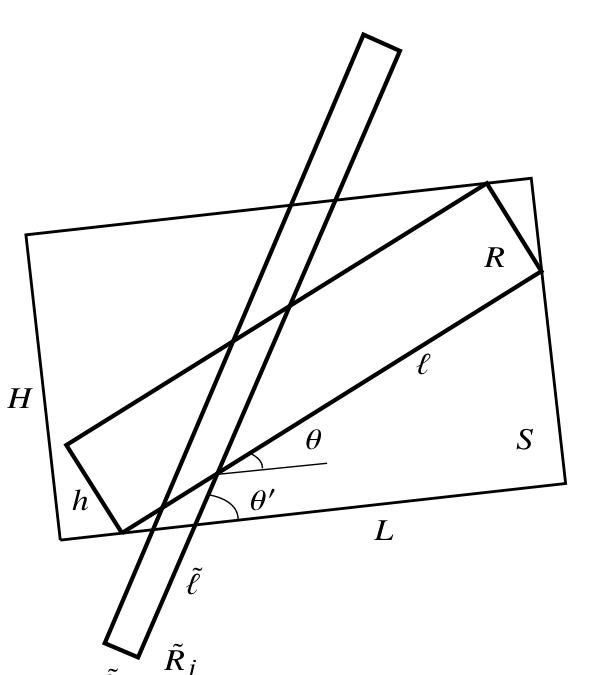
\includegraphics[width=0.38\textwidth]{figs/fig-2-6.png}
\caption{包络矩形.}
\label{fig:2.6}
\end{figure}

然后, 必要时把 $S$ 膨胀, 可以假设 $\tilde{R}_{j}$ 与 $S$ 同心. 关键在于
\begin{equation}\label{eq:2.9}
  \frac{\mu(\tilde{R}_{j}\cap S)}{\mu(S)}\geq\frac{\mu(\tilde{R}_{j}\cap R)}{\mu(R)}.
\end{equation}
事实上,
\begin{align*}
  \frac{\mu(\tilde{R}_{j}\cap S)}{\mu(S)}\sim\frac{\widetilde{h}\,H/\theta^{\prime}}{h\,L}
  =\frac{\widetilde{h}}{L\,\theta^{\prime}},\qquad
  \frac{\mu(\tilde{R}_{j}\cap R)}{|R|}\sim\frac{\widetilde{h}\,h(\theta^{\prime}-\theta)}{h\,l}
  =\frac{\widetilde{h}}{l\,(\theta^{\prime}-\theta)},
\end{align*}
而我们的不等式 \eqref{eq:2.9}, 考虑到 $l \sim L$, 为
\begin{align*}
  \frac{1}{\theta^{\prime}}\geq\frac{1}{\left(\theta^{\prime}-\theta\right)},
  \qquad\text{即}\qquad
  \theta^{\prime}-\theta\geq c\,\theta^{\prime},
\end{align*}
在我们 $\theta_k = 2^{-k}$ 的情形, 它取 $c = 1/2$ 时成立. （若 $\theta_k = (1 - \varepsilon)^k$, 则取 $c = \varepsilon$.）于是在 \eqref{eq:2.9} 中对 $j$ 求和, 有
\begin{align*}
  \frac{1}{\mu(S)}\int_{S}\sum_{\substack{\tilde{R}_{j}\ \text{在}\ R\ \text{之前}}}\chi_{\tilde{R}_{j}}
  \geq\frac{1}{\mu(R)}\int_{R}\sum_{\substack{\tilde{R}_{j}\ \text{在}\ R\ \text{之前}}}\chi_{\tilde{R}_{j}}
  \geq\frac{1}{2}\,c.
\end{align*}
换句话说, 在 $\bigcup_{j}R_{j}$ 上有
\begin{align*}
  M_{2}\Big(\sum_{j}\chi_{R_{j}}\Big)>\frac{1}{2}\,c,
\end{align*}
由 $M_{2}$ 的有界性, 并由 \eqref{eq:2.9}, 可见
\begin{align*}
  \mu\Big(\bigcup_{j}R_{j}\Big)\lesssim\Big\|\sum_{j}\chi_{\tilde{R}_{j}}\Big\|_{2}^{2}
  \lesssim\mu\Big(\bigcup_{j}\tilde{R}_{j}\Big).
\end{align*}
这里我们控制算子 $\mathcal{M}$ 于 $M_2$, 其方式与先前用 $M_{n-1}$ 控制 $M_n$ 完全一样. 而 $\mathcal{M}$ 是三参数极大算子, $M_2$ 是两参数算子.

最后应该注意, 如前, 这个覆盖引理蕴含 $\mathcal{M}$ 的极大定理, 正如所断言的那样. 事实上, 假设已经证明: 给定 $\{R_k\}$, 存在子列 $\{\tilde{R}_k\}$, 使得
\begin{align*}
  \mu\Big(\bigcup_{k}\tilde{R}_{k}\Big)\gtrsim\mu\Big(\bigcup_{k}R_{k}\Big),
\end{align*}
\begin{enumerate}
\item[(2)] $\Big\|\sum_{k}\chi_{R_k}\Big\|_{p'} \lesssim \mu\Big(\bigcup_{k} R_k\Big)^{1/p'}$, 其中 $1/p + 1/p' = 1$.
\end{enumerate}
则
\begin{align*}
  \mu(\{\mathcal{M}f>\alpha\})\leq\left(c\,\frac{\left\|f\right\|_{p}}{\alpha}\right)^{p}.
\end{align*}
事实上, 由定义存在 $\{R_{k}\}$, 使
\begin{align*}
  \{\mathcal{M}f>\alpha\}\subseteq\bigcup_{k}R_{k},\qquad
  \frac{1}{\left|R_{k}\right|}\int_{R_{k}}\left|f\right|>\alpha\quad\text{对所有 } k.
\end{align*}
由覆盖引理选取类 $\{\tilde{R}_{k}\}$. 则
\begin{align*}
  |\tilde{R}_{k}|\leq\frac{1}{\alpha}\int_{\tilde{R}_{k}}|f|,
\end{align*}
于是
\begin{align*}
  \mu\Big(\bigcup_{k}\tilde{R}_{k}\Big)
  &\leq\frac{1}{\alpha}\int f\sum_{k}\chi_{\tilde{R}_{k}}
  \leq\frac{1}{\alpha}\left\|f\right\|_{p}\left\|\sum_{k}\chi_{R_{k}}\right\|_{p^{\prime}}
  \leq\frac{C}{\alpha}\left\|f\right\|_{p}\,\mu\Big(\bigcup_{k}R_{k}\Big)^{1/p^{\prime}}\\
  &\leq C^{\prime}\left\|f\right\|_{p}\,\mu\Big(\bigcup_{k}\tilde{R}_{k}\Big)^{1/p^{\prime}},
\end{align*}
把两边除以 $\mu\bigl(\bigcup_{k}\tilde{R}_{k}\bigr)^{1/p'}$, 即得关于 $\mu(\{\mathcal{M}f > \alpha\})$ 的估计.

上述论证给出了 $\R^2$ 中一般\newterm{lacunary}{缺项的}{lacunary}\newterm{direction-set}{方向集}{set of directions}的类似定理, 即满足 $\theta_k \searrow \theta$ 且对 $k = 1, 2, 3, \ldots$
\begin{align*}
  \frac{\theta_k - \theta_{k+1}}{\theta_{k+1} - \theta_{k+2}} \geq \rho > 1
\end{align*}
的集合 $\{\theta_k\}$.

此外, 结果对一般 $p > 1$ 成立. 即, 对 $p > 1$ 有不等式
\begin{align*}
  \mu\{\mathcal{M}f>\alpha\}\leq c_{p}(\rho)\,\alpha^{-p}\|f\|_{p}^{p},
\end{align*}
见 \cite{b50}. 但那里的证明不循本章的至上主义方法.

% ================================================================
% 编号审计 (第 2 章):
%   lemma     lem:2.1  → 引理 2.1  (§2.1)
%   lemma     lem:2.2  → 引理 2.2  (§2.1)
%   lemma     lem:2.3  → 引理 2.3 (Calderón–Zygmund) (§2.1)
%   definition def:2.4 → 定义 2.4  (§2.2)
%   theorem   thm:2.5  → 定理 2.5  (§2.2)
%   remark    rem:2.6  → 注 2.6    (§2.2)
%   theorem   thm:2.7  → 定理 2.7  (§2.3)
%   theorem   thm:2.8  → 定理 2.8  (§2.4)
%   definition def:2.9 → 定义 2.9  (§2.4)
%   lemma     lem:2.10 → 引理 2.10 (§2.4)
%   theorem   thm:2.11 → 定理 2.11 (§2.4)
%   公式: eq:2.1 (Hardy–Littlewood 极大函数), eq:2.2 (弱型不等式),
%         eq:2.3 (稀疏性), eq:2.4 (指数估计), eq:2.5 (切片估计),
%         eq:2.6 (选择过程), eq:2.7 (双指数恒等式), eq:2.8 (重叠比),
%         eq:2.9 (包络矩形比)
%   无编号 Claim 用 claim* 环境 (证明内嵌于定理 2.8 的证明).
%   \cite 使用: b14 b41 b46 b48 b50 b51 b52 b54 b56 b57
% ================================================================
